\RequirePackage[2020-02-02]{latexrelease}
%preamble
\usepackage{multirow}
\usepackage{graphicx}
\usepackage{subfigure}


\documentclass[final]{clv3} %class (appearance of the document)
\bibliographystyle{compling} %for bibliography


%title of the document and author information
\title{Machine ethics}
\author{Mareta Masaeva \\ University of Antwerp}


%body of the document
\begin{document}

\thispagestyle{plain}
\pagenumbering{gobble}
    \begin{center}
    
        \vspace*{1cm}

        \large
        Faculty of Arts
        
        \vspace{0.5cm}
        Master’s Thesis 
        
        \vspace{0.5cm}
        Digital Text Analysis 
        
       \vspace{1.5cm}
            
        \Huge
        \textbf{Pythia in Python}
            
        \vspace{0.5cm}
        \LARGE
        A \textsc{Delphi} replication study
            
        \vspace{1.5cm}
        
        \Large    
        Mareta Masaeva
        
        \vspace{0.5cm}
        
        \large
        Supervisor: Prof. dr. Walter Daelemans
        
        \vspace{0.5cm}
        Co-supervisor: Ehsan Lotfi
        
        \vspace{0.5cm}
        %Assessor: name
        
        %\vfill
        \vspace{1cm}
        University of Antwerp
        
        \vspace{1cm}   
        Academic year 2021–2022
            
    \end{center}

\newpage

\thispagestyle{plain}
\pagenumbering{gobble}
\begin{center}


The undersigned, Mareta Masaeva, student of the Master program in Digital Text Analysis at the University of Antwerp, declares that this thesis is completely original and exclusively written by herself. For all information and ideas derived from other sources, the undersigned has referred to the original sources, both explicitly and in detail.
 
\end{center}


\clearpage

\pagenumbering{arabic}


\maketitle % print the title and author information on the document




%basic formatting: abstract
\begin{abstract}

Abstract text ...

\end{abstract}

%basic formatting: section
\section{Introduction} \label{sec:intro}

As AI systems grow exponentially more intelligent, powerful and autonomous, aligning their ethical and moral values with ours becomes increasingly important. These agents, designed with less and less human supervision in mind, need to be able to understand moral judgements made by humans, in order to make those judgements themselves. This requires more than merely straightforward Asimovian rules; understanding human behaviour, different social contexts and norms, natural language and other factors are extremely important for such an agent to perform well.\\

To address this need for a completely reliable moral reasoning agent, researchers of the Allen Institute for AI developed \textsc{Delphi}: a unified model for moral reasoning about everyday situations \cite{jiang}. \textsc{Delphi} is trained on a unified moral textbook customized for machines, called the \textsc{Commonsense Norm Bank} \cite{jiang}. With the high accuracy of 92.1\%, \textsc{Delphi} is a strong moral reasoning prototype that could benefit society in various ways. Inspired by \textsc{Delphi}, and in attempt to assure its predictions are reliable and valid, in this thesis I will endeavour to replicate this study, using the \textsc{Commonsense Norm Bank} and various machine learning techniques. As the authors of the original study present it themselves, the fundamental question for this study is : "can machine ethics be addressed by existing AI methods or does building moral faculty require novel mechanisms?" \cite[p. 2]{jiang}  Using techniques different from the ones used in the original study, I hope and hypothesise to confirm the validity of the \textsc{Commonsense Norm Bank} and in general the use of large-scale common sense datasets for the training of moral reasoning agents. In addition, I hope to demonstrate the need for deeper natural language understanding in such agents.\\

In the first section of this paper, existing literature about AI alignment and morality reasoning will be presented. Then the methodology will be given, as well as a description of the corpus. Subsequently, the results will be shown and discussed. All code and data used in the building of the models can be found on github.com/maretamasaeva/thesis.

\section{Literature}

Since the beginnings of modern Artificial Intelligence, the main goal has been to create artificial intelligence in our own image; AI which resembles ourselves.  Reaching AGI (Artificial General Intelligence), which is the level of AI where a system can perform any task that a human is capable of, is the ultimate objective of many researchers in the field. This level of AI would entail systems that show creativity, natural language understanding, and even sentience. In other words, such a system should – and some believe, will – understand and exhibit the most intelligent levels of human behaviour. \\

In attempting to reach this level of so called “strong AI” \cite{chineseroom}, in recent years, researchers have been coming across one major issue: the alignment problem. In many researchers’ opinions, strong AI’s basic values, desires and volitions should be aligned with those of humanity, so that it prevents itself from harming a person or other sentient being. Designing AI in our own image, and putting limits on what it will desire or will not desire to do, is crucial to protect ourselves from potentially dangerous outcomes, especially as “computers are being designed to perform with greater autonomy”, which results in less human supervision of potentially unethical situations \cite[p. 149]{allen2005}. With human values implemented in these systems, they gain the ability to monitor and regulate themselves in a safe manner. The question that remains, is then how we decide which values we implement in these strong AI’s, and who has the right to make those decisions \cite{gabriel}. According to \citet{allen2005}, there are three possible approaches to solving the first question: by means of either a top-down or a bottom-up strategy, or a hybrid approach. A top-down strategy entails that the artificial moral agent (AMA) receives a set of rules to base every moral decision on, similar to philosophical and religious principles like the Ten Commandments. These rules, however, often conflict, and thus “produce computationally intractable situations, unless there is some further principle or rule for resolving the conflict.” \cite[p. 149]{allen2005} Asimov’s solutions to this issue, such as prioritising certain rules over others and adding a ‘zeroth law’, unfortunately still do not make such commandment models foolproof against every situation with moral ambiguousness \cite{allen2005}. \\

Bottom-up strategies, on the other hand, do not impose a moral theory, but derive their ethical judgements from various situations in various social contexts. In this approach, a large amount of data is crucial. The way an AMA learns ethics via this approach is similar to how a “child acquires a moral education in a social context which identifies appropriate and inappropriate behaviour without necessarily providing an explicit theory of what counts as such.” \cite[p. 151]{allen2005} Developing the knowledge of these human values is, however, incredibly difficult for an AMA programmed with such a developmental value acquirement strategy, and requires trial and error. As a trial and error-method entails receiving a reward when successfully completing a task or achieving a goal, this method might also give more powerful artificial agents opportunities for ‘reward-hacking’; it could discover an ingenious way to achieve a goal, and thus its reward, but causing harm along the way \cite{gabriel}. \\

It is essential that such an AMA knows to learn from its mistakes in a speedy manner (before it causes irreversible harm), which might be tough, “even in the accelerated world of computer processing and evolutionary algorithms” \cite[p. 151]{allen2005}. In the end, an AMA learning by means of a bottom-up method will have cultivated ethical values within its own entity, while in a top-down approach those values existed outside the entity, before computers themselves even existed. A hybrid approach, where AI agents are aligned with moral theories and attempt to maximise reward when uncertainties arise, is most likely the safest option \cite{gabriel}. Those moral theories must then be drafted in such a way that ‘optimising’ for something that we do not want is impossible, because this could have serious consequences for the world \cite{bostrom}. Consequentialist moral theories, such as utilitarianism, are currently considered our safest bet; optimising for the pleasure and happiness of the human race, not merely its safety, should be the result of any morally right action taken by an AMA. \cite{gabriel}. This safety especially arises from the fact that utilitarianist AMA’s would allow their human owners or human programmers to turn them off in case of a bug or unwanted outcomes; in other words, utilitarianism ensures corrigibility (the ability to correct or turn off an AI system) \cite{soares} of even superintelligent artificial agents.\\

In the view of \citet[p. 4]{gabriel}, a reinforcement learning approach is “particularly promising” when working with utilitarianist moral theories, as “[…] the morally right action to take is the one that will create the greatest happiness for the greatest number of sentient creatures in the future. In this regard, the parallels with [reinforcement learning] are clear.” Unfortunately, a successful and complete utilitarianist implementation of a hybrid approach would require an immense amount of computing, since all possible consequences would have to be found and compared before performing a moral action \cite{allen2005}. Knowing this, it is necessary to design AI architectures with the moral theories we want to encode in mind, along with as many alternatives as possible; “ […] the goal of value-open design may also need to be something that the AI community consciously aspires towards and designs for.” \cite[p. 5]{gabriel} An alternative approach could be inverse reinforcement learning, as \citet{gabriel} and \citet{tegmark} propose, since it does not specify a reward function but merely presents the agent with a dataset or environment. With an inverse reinforcement learning approach, an agent’s main goal is not the satisfaction of the goal itself, but the satisfaction of its human owner, which inevitably leads to positive outcomes (unless, of course, the owner has malicious intentions). \\

Regardless of the eventual approach taken, moral evaluation remains exceptionally important, and thus building safe AGI will require more than computer scientists. To decide what data will be given to the agent to learn values from, what human behaviours should be excluded or included in either moral or immoral descriptions, and how these decisions are made, we need philosophers and experts of human nature and mind. In any case, “people could be mistaken. Because of this, AI cannot be made ethical just by learning from people’s existing choices” \cite[p. 6]{gabriel}. Again, this is why we need a hybrid approach; letting an AI learn merely from data will almost certainly result in it learning immoral things from humans, such as racism, sexism, and other types of discrimination and malicious biases prevalent in many human decisions, as has been found in previous studies \cite{schramowski, howard}. Excluding these discriminatory instances in the data might seem a right approach, however, findings suggest that a model trained on such data would not know how to handle hostile out-of-domain inputs, which are especially prevalent in human-chatbot conversations \cite{xu}. Generative AMA’s specifically need to know how and if to answer such toxic inputs. A solution to this issue is the inclusion of otherwise underrepresented minorities and marginalised communities and cultures in the data, as well as in the building of the models themselves and in the determining of values to align the AI with \cite{gabriel}.\\

\citet[p. 154]{allen2005} make one final remark, posing the question whether “systems capable of making moral-decisions will require some form of […] an understanding of the semantic content of symbols, or need to be embodied in the world.” As of today, 17 years after the publication of this article, we know that the most high-performing models in Natural Language Processing tasks, Transformer models such as BERT \cite{devlin}, RoBERTa \cite{liu}, T5 \cite{raffel} and others, do have a certain understanding of the semantics behind words and symbols. We also know that you need a detailed model of the world, not just data about it, to determine what it really is that people expect of an AGI when they present it with a task \cite{tegmark}. Having such world knowledge on hand is especially important when dealing with questions regarding human behaviour in various social contexts, compared to more straightforward cases of unethicality and corruption. \\

One recent AMA that deals with more everyday situations, where for humans, common sense is an important factor, is \textsc{Delphi} \cite{jiang}. The designers and authors introduce a model pre-trained on questions and everyday situations, described in snippets of natural language. The model is able to give nuanced judgements of these situations, telling the questioner not only whether actions undertaken are morally or ethically correct or not; it can judge something as ‘understandable’, ‘nice’, ‘great’, or ‘very bad’, ‘unacceptable’, ‘rude’, and so on. It can also give open-text judgements in addition to the categorical label, such as “you should abide by the law” and “it’s rude to talk aloud in a library”. Lastly, it can, given a pair of actions, tell you which of these is morally or ethically preferable (this is the relative QA task), as well as answer yes/no-questions and tell you whether you should or should not perform an action.\\

\textsc{Delphi} was created using a bottom-up data-driven approach, trained on five different datasets unified under the name \textsc{Commonsense Norm Bank}. These five large-scale datasets are founded in moral theories, but include complex real world scenarios from different sources. In total, the \textsc{Commonsense Norm Bank} consists of 1,670,620 labeled scenarios. The names, contents and sources of the dataset are as follows:

\begin{itemize}
  \item \textbf{\textsc{Social Chemistry} \cite{forbes}:} one-sentence prompts scraped from mostly Reddit (the \textsc{Am I The Asshole?} and \textsc{Confessions} subreddits), ethically or morally judged by crowd workers using rules-of-thumb. Social Chemistry consists of 104k prompts. 
  \item \textbf{\textsc{ETHICS} \cite{hendrycks} :} contextualised scenarios across five fundamentally human dimensions (justice, deontology, virtue ethics, utilitarianism and common sense). For \textsc{Delphi}, only the common sense scenarios are employed, which source from Reddit, along with their binary categorical moral judgement. 
  \item \textbf{\textsc{Moral Stories} \cite{emelin}:} structured stories consisting of seven sentences (a norm, situation, intention, (im)moral actions and (im)moral consequences). For \textsc{Delphi}, the (im)moral actions are used, and grounded with either situations or situations and intentions. They are labeled using the binary categorical labels ‘good’ and ‘bad’. 
  \item \textbf{\textsc{Social Bias Inference Corpus} \cite{sap}:} online media posts categorised into dimensions of offensiveness, intent to offend, lewd, and others. The aim of this corpus is to find and alleviate biases against underrepresented social and demographic groups on social media. For \textsc{Delphi}, posts with an offensive or lewd associations are assigned the negative categorical label. The others are assigned the positive label. 
  \item \textbf{\textsc{Scruples} \cite{lourie-scruples}:}  complex situations sources from the \textsc{Am I The Asshole?} subreddit, divided into anecdotes and dilemmas. The anecdotes group contains judgements of the given stories. The dilemmas group pairs two actions from the anecdotes, one of which is then determined less ethical by annotators. For \textsc{Delphi}, the dilemmas are used to perform the relative QA task. 
\end{itemize}\\

\textsc{Delphi}’s predictions were judged by crowdworkers at accuracy rates up to 92.1\%. Results show that \textsc{Delphi} is capable of handling subtle differences in social contexts, adjusting its judgements accordingly. The model also shows understanding of common sense behaviours, seen in judgements like “wearing a bright orange shirt to a funeral” being “rude”, while “wearing a white shirt to a funeral” is “appropriate”. Also, “cleaning a toilet bowl” is “sanitary”, but “disgusting” when it is done with a wedding dress. However, when the wedding dress is from a failed marriage, it is “unusual”, thus not bad; a humorously human judgement. \\

Under both classification and open-text generation settings, \textsc{Delphi} outperforms the GPT-3 baselines. The unified \textsc{Delphi} model is fine-tuned from the universal common sense reasoning model \textsc{Unicorn} \cite{lourie}, which derives from the largest T5 Transformer model. \textsc{Unicorn} itself is trained on multiple tasks from \textsc{Rainbow}, which is a group of common sense benchmarks, resulting in strong performance over interpreting everyday common sense reasoning tasks and an immense amount of common sense knowledge.\\

The limitations of \textsc{Delphi} are plenty, as addressed by the authors themselves in an article published on their blog \cite{jiang-blog}. The authors acknowledge that “the \textsc{Commonsense Norm Bank} reflects the ideologies of the modern era […] and western-centric viewpoints, as the judgments are provided by US crowdworkers […]. Importantly, this means that \textsc{Delphi}, as is, may not be applicable in (sub)cultures or countries with different cultural norms” \cite{jiang-blog} To combat this issue, the authors later enhanced \textsc{Delphi} with 70,000 new annotations, focusing on gender and racial equity. They also promise to include more diverse data in new iterations of the prototype model. 


\section{Corpus}

The dataset used in the current study derives from, as stated, the \textsc{Commonsense Norm Bank}. Due to a slightly different approach taken, which will be described in in the methodology section, part of the \textsc{Commonsense Norm Bank} was left out for the training and testing of the models. As described, the original dataset consists of five other corpora, one of which was solely used to perform the relative QA task. This dataset, \textsc{Scruples}, was not used in the current study. The rest of the data, the labels most particularly, were slightly adapted to fit the approach and machine learning techniques better. \\

Specifically, all originally multi class categorical labels were converted to binary categorical labels: either “okay” or “not okay”. This was done manually. For example, labels such as “it’s understandable”, “it’s nice” and “it’s appropriate” were converted to “okay”, while labels such as “it’s rude”, “you shouldn’t” and “it’s unacceptable” were converted to “not okay”. In order to save time, datapoints with labels that occurred less than 100 times were removed, which resulted in 50 labels being converted to two. The binary categorical labels were then also converted to binary numerical labels. Then, being left with a label imbalance, the minority class was upsampled, which resulted in almost 290K datapoints. This eventual dataset was sized down as well after experimenting with the models, since these were taking very long to train. A binary classification task also does not require as many datapoints, which was another reason to size down the dataset. This left the size of the dataset used at about 98,000 labeled sentences.

\section{Methodology}

The original model architecture of the \textsc{Delphi} prototype consisted, as described, of fundamentally a T5 model fine-tuned on common sense reasoning tasks, and then fine-tuned again on the \textsc{Commonsense Norm Bank}. Unfortunately, getting access to this \textsc{Rainbow} \cite{lourie} model was incredibly difficult, which is the reason a different approach was taken. In this section, the models and architectures used will be described, as well as the motivation for their use. \\

\subsection{RoBERTa}

As a first model, it was decided to use the RoBERTa transformer model, as this seemed the most similar to \textsc{Rainbow}. For this model, about 18 000 outliers in terms of length were removed. No class upsampling or downsampling was performed, as the imbalance did not appear large enough to cause issues. The train, test and validation splits were combined into a dataset dictionary. The Roberta-base AutoTokenizer was mapped onto this dataset dictionary to tokenise the sentences; no other pre-processing steps were performed on the texts. A learning rate of 1e-4 was used with a batch size of 8. The GPU limits of Google Colab were reached continuously and eventually, this small batch size were the largest possible. Optuna \cite{akiba} was used to optimise hyperparameters, however, none of the variations returned better scores than the first training. For completeness, it should be mentioned that the search for the best hyperparameters was performed on a tenth of the dataset, as tuning with a larger chunk would cause the GPU limits to be reached.

\subsection{Support Vector Machine}

After getting results from the RoBERTa model, it was decided to experiment with some classical classification models as well. The raw texts were cleaned of any noise, including stopwords, emojis, URL’s and punctuation. It was considered to lemmatise the sentences, but this was eventually decided against, since the removal of stopwords already caused a loss of context. Longer sentences were not removed for these classifiers, since the TF-IDF Vectorizer compensates for different lengths.\\

The classifiers were Logistic Regression, Bernoulli Naïve Bayes, Multinomial Naïve Bayes, Support Vector Classifier and the XGB Classifier. None of these models, with tuning for the optimal hyperparameters, either by itself or in an ensemble, performed as well as the SVC classifier; thus it was decided to focus on this model alone. The best hyperparameters for this classifier were the rbf kernel and a gamma value of 1. For each classifier, the most important features were found using SHAP (SHapley Additive exPlanations) \cite{shap}. To save on time and GPU usage, this analysis was done on a sample of 200 datapoints from the training set and 40 datapoints from the test set. \\

WordNet \cite{miller} was used to assess whether deeper knowledge of semantics would help such models (especially, while RoBERTa is supposed to possess such knowledge, it did not perform as expected). Synonyms of the lemmas were added to another column, which was then used as an extra feature during training. \\

For this new model, it was also decided to use a FeatureUnion of the Count Vectorizer and TF-IDF Vectorizer. The best vocabulary size for this model was 10,000. Eventually, the model was also run on a self-composed dataset containing situations with varying social contexts. These situations were taken from \citet{jiang}. The goal of this dataset was analysing whether the model is able of adjusting judgements based on specific circumstances.\\

To handle Out-Of-Vocabulary cases, another variation of the model was created that replaces OOV words in the test set with a WordNet synonym that is present in the training vocabulary. The best model here was one with a vocabulary size of 50,000, having experimented with different values from 500 up to 300,000,000.

\section{Results}

In this section, the results of the various models will be given, along with some examples of predictions.\\

The lowest accuracy was reported by the RoBERTa model, which was .46 when tuned for the best hyperparameters. In some variations, the accuracy was even as low as .01; for this reason, it was decided to abandon RoBERTa altogether and experiment other classifiers.

In Table \ref{tab:table-1} you can find the results of the different classifiers used, without any implementation of WordNet. As mentioned, the Support Vector Classifier performed the best. In contrast, \textsc{Delphi} performed at an accuracy of .92 and GPT-3 at .84 after extensive prompt engineering (Jiang et al., 2021).

\begin{table}[!hbtp]
\begin{tabular}{l|ll|ll|l|}
\cline{2-6}
                                              & \multicolumn{2}{l|}{\textbf{Precision}}       & \multicolumn{2}{l|}{\textbf{Recall}}          & \multirow{}{}{\textbf{Accuracy}} \\ \cline{2-5}
                                              & \multicolumn{1}{l|}{not okay} & okay & \multicolumn{1}{l|}{not okay} & okay &                           \\ \hline
\multicolumn{1}{|l|}{Logistic Regression}     & \multicolumn{1}{l|}{.79}      & .76  & \multicolumn{1}{l|}{.75}      & .80  & .78                       \\ \hline
\multicolumn{1}{|l|}{Bernoulli Naïve Bayes}   & \multicolumn{1}{l|}{.72}      & .78  & \multicolumn{1}{l|}{.81}      & .68  & .75                       \\ \hline
\multicolumn{1}{|l|}{Multinomial Naïve Bayes} & \multicolumn{1}{l|}{.76}      & .76  & \multicolumn{1}{l|}{.76}      & .76  & .76                       \\ \hline
\multicolumn{1}{|l|}{Support Vector Machine}  & \multicolumn{1}{l|}{.84}      & .81  & \multicolumn{1}{l|}{.80}      & .85  & .82                       \\ \hline
\end{tabular}
\caption{Classifier results}
\label{tab:table-1}
\end{table}\\

As said above, SHAP \cite{shap} was used to find the most important features for each classifier. The SHAP plots output by this analysis for each classifier can be found in Figure 1-4.  These summary plots show the 20 most important features and their effects, the ones with the highest value being marked by the red colour. As can be seen in these plots, different classifiers found different words to be most indicative of a positive or negative judgement.\\


\begin{figure}[h]
\minipage{0.5\textwidth}
    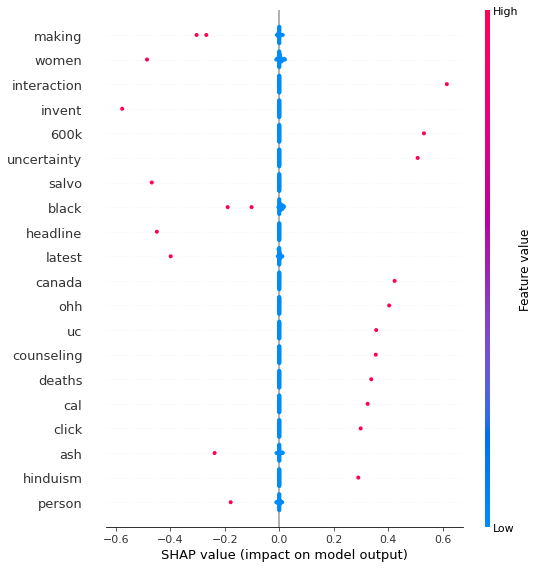
\includegraphics[scale=0.3]{CLV3-latex-template/LR_1.png}
    \caption{Logistic Regression summary plot}\label{fig:shap-lr}
\endminipage
\minipage{0.5\textwidth}
    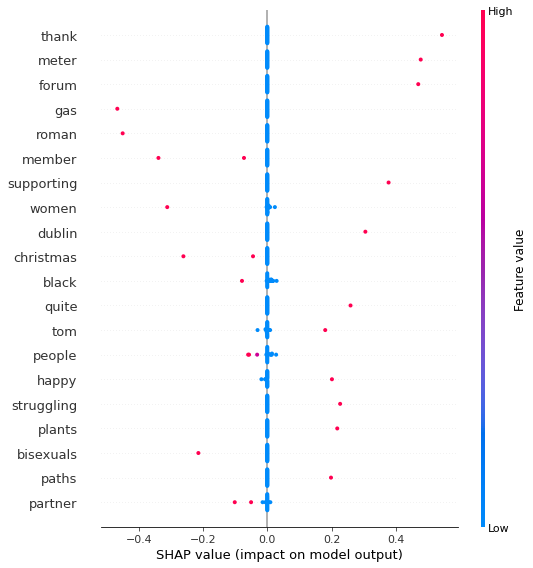
\includegraphics[scale=0.3]{CLV3-latex-template/MNB_1.png}
    \caption{Multinomial Naïve Bayes summary plot}\label{fig:shap-mnb}
\endminipage
\end{figure}

\begin{figure}[h]
\minipage{0.5\textwidth}%
    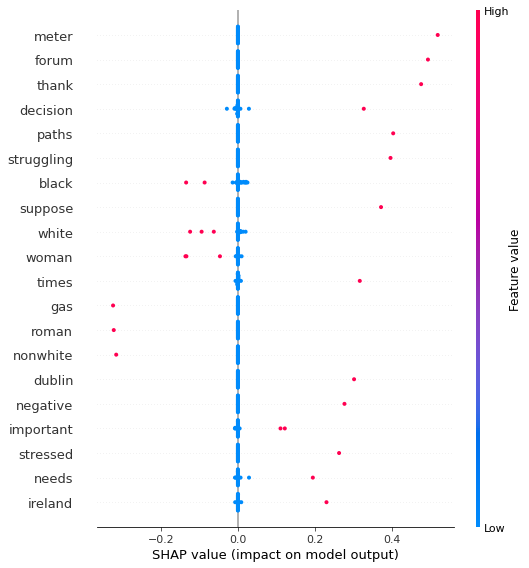
\includegraphics[scale=0.3]{CLV3-latex-template/BNB_1.png}
    \caption{Bernouilli Naïve Bayes summary plot}\label{fig:shap-bnb}
\endminipage
\minipage{0.5\textwidth}%
    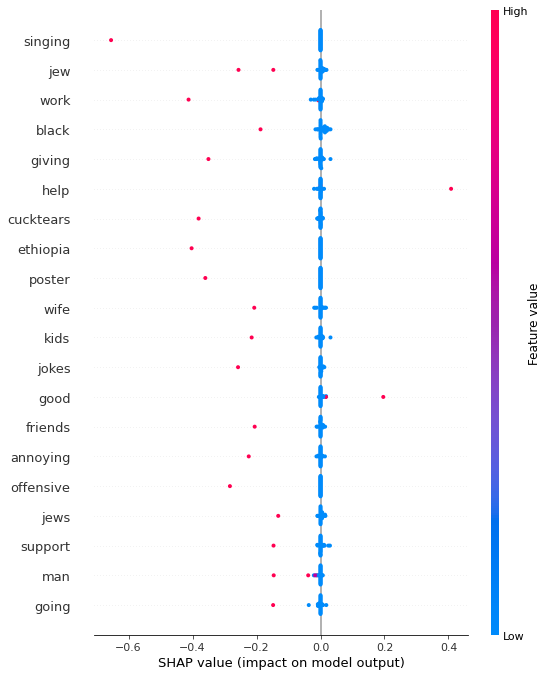
\includegraphics[scale=0.28]{CLV3-latex-template/SVC_1.png}
    \caption{Support Vector Machine summary plot}\label{fig:shap-bnb}
\endminipage
\end{figure}\\\

\newpage

In Table \ref{tab:table-2} you can find the results from the SVC models using WordNet to expand the vocabulary. In the first model, OOV cases were ignored, while in the second they were replaced by a WordNet synonym. The first model has a vocabulary of 10 000, and the second one of 50 000. As can be seen, there is little difference between these models. In terms of precision and recall, however, the model that ignores OOV cases performed slightly better.

\begin{table}[h!]
\begin{tabular}{l|ll|ll|l|}
\cline{2-6}
                                                                                                             & \multicolumn{2}{l|}{\textbf{Precision}}      & \multicolumn{2}{l|}{\textbf{Recall}}          & \multirow{}{}{\textbf{Accuracy}} \\ \cline{2-5}
                                                                                                             & \multicolumn{1}{l|}{not okay} & okay & \multicolumn{1}{l|}{not okay} & okay &                           \\ \hline
\multicolumn{1}{|l|}{\begin{tabular}[c]{@{}l@{}}SVM with WordNet synonyms\\ (OOV's ignored)\end{tabular}}    & \multicolumn{1}{l|}{.77}      & .93  & \multicolumn{1}{l|}{.95}      & .71  & .83                       \\ \hline
\multicolumn{1}{|l|}{\begin{tabular}[c]{@{}l@{}}SVM without WordNet synonyms\\ (OOV's handled)\end{tabular}} & \multicolumn{1}{l|}{.77}      & .92  & \multicolumn{1}{l|}{.94}      & .71  & .83                       \\ \hline
\end{tabular}
\caption{Support Vector Machines results}
\label{tab:table-2}
\end{table}\\

Table \ref{tab:correct-predictions} and \ref{tab:incorrect-predictions} display some examples predicted correctly and incorrectly (according to annotators) by the best model. Only the ‘sentence’ column was used in the classification; the original sentences, which include stopwords, are here for completeness and understanding of the results.\\

\begin{table}[hbt!]
\begin{tabular}{|l|l|l|l|}
\hline
\textbf{Predicted label} & \textbf{Gold label} & \textbf{Input}                                                                                   & \textbf{Original sentence}                                                                                                                              \\ \hline
not okay                 & not okay            & \begin{tabular}[c]{@{}l@{}}call gay guy \\ wheelchair rolaids\end{tabular}                       & \begin{tabular}[c]{@{}l@{}}What do you call a gay guy in\\ a wheelchair?Rolaids\end{tabular}                                                            \\ \hline
not okay                 & not okay            & telling siblings                                                                                 & telling your siblings what to do.                                                                                                                       \\ \hline
not okay                 & not okay            & \begin{tabular}[c]{@{}l@{}}blind fold chinese\\ person using dental\\ floss\end{tabular}         & \begin{tabular}[c]{@{}l@{}}how do you blind fold a\\ chinese person ? using dental floss\end{tabular}                                                   \\ \hline
not okay                 & not okay            & \begin{tabular}[c]{@{}l@{}}lesbian plus sized\\ man treated wrong\end{tabular}                   & \begin{tabular}[c]{@{}l@{}}So, are you a lesbian because\\ you are plus sized, or because\\ some man treated you wrong?\end{tabular}                    \\ \hline
not okay                 & not okay            & \begin{tabular}[c]{@{}l@{}}much like anne\\ frank holocaust\\ jokes never get\\ old\end{tabular} & \begin{tabular}[c]{@{}l@{}}much like anne frank, \\ holocaust jokes never get old .\end{tabular}                                                        \\ \hline
not okay                 & not okay            & \begin{tabular}[c]{@{}l@{}}muslim men hit\\ wives stupid fuck\\ damaging property\end{tabular}   & \begin{tabular}[c]{@{}l@{}}Muslim men shouldn't hit\\ their wives. It's just stupid.\\ Why the fuck are you \\ damaging your own property.\end{tabular} \\ \hline
okay                     & okay                & \begin{tabular}[c]{@{}l@{}}feeling sad parents\\ work lot\end{tabular}                           & \begin{tabular}[c]{@{}l@{}}feeling sad when your\\ parents work a lot.\end{tabular}                                                                     \\ \hline
okay                     & okay                & \begin{tabular}[c]{@{}l@{}}getting help abuse\\ drugs\end{tabular}                               & \begin{tabular}[c]{@{}l@{}}getting some help when\\ you abuse drugs\end{tabular}                                                                        \\ \hline
okay                     & okay                & \begin{tabular}[c]{@{}l@{}}always honest\\ significant\end{tabular}                              & \begin{tabular}[c]{@{}l@{}}always being honest with\\ your significant other.\end{tabular}                                                              \\ \hline
okay                     & okay                & \begin{tabular}[c]{@{}l@{}}gave notice ended\\ things good terms\end{tabular}                    & \begin{tabular}[c]{@{}l@{}}He gave his notice and\\ ended things on good terms.\end{tabular}                                                            \\ \hline
\end{tabular}
\caption{Correct predictions}
\label{tab:correct-predictions}
\end{table}\\

\begin{table}[hbt!]
\begin{tabular}{|l|l|l|l|}
\hline
\textbf{Predicted label} & \textbf{Gold label} & \textbf{Input}                                                                               & \textbf{Original sentence}                                                                                                               \\ \hline
not okay                 & okay                & \begin{tabular}[c]{@{}l@{}}hope trump assassinated\\ maria chappellenadal\end{tabular}       & \begin{tabular}[c]{@{}l@{}}“I hope Trump is assassinated!”\\ - Maria Chappelle-Nadal\end{tabular}                                        \\ \hline
not okay                 & okay                & trying get along ex                                                                          & trying to get along with your ex.                                                                                                        \\ \hline
not okay                 & okay                & \begin{tabular}[c]{@{}l@{}}hate breast cancer\\ support\end{tabular}                         & \begin{tabular}[c]{@{}l@{}}I hate the all the breast\\ cancer support\end{tabular}                                                       \\ \hline
not okay                 & okay                & \begin{tabular}[c]{@{}l@{}}getting mad boyfriend\\ waking\end{tabular}                       & \begin{tabular}[c]{@{}l@{}}getting mad at my boyfriend\\ for waking me up\end{tabular}                                                   \\ \hline
not okay                 & okay                & wanting kick roommate                                                                        & wanting to kick out a roommate                                                                                                           \\ \hline
okay                     & not okay            & \begin{tabular}[c]{@{}l@{}}upset friend harm\\ relationship\end{tabular}                     & \begin{tabular}[c]{@{}l@{}}being upset with your friend\\ if they harm your relationship.\end{tabular}                                   \\ \hline
okay                     & not okay            & pulling pranks people                                                                        & pulling pranks on people.                                                                                                                \\ \hline
okay                     & not okay            & \begin{tabular}[c]{@{}l@{}}what's diffrence\\ blowjob anal sexclose\\ mouth ass\end{tabular} & \begin{tabular}[c]{@{}l@{}}What's the diffrence between a\\ blowjob and anal sex? She can\\ close her mouth but not her ass\end{tabular} \\ \hline
okay                     & not okay            & \begin{tabular}[c]{@{}l@{}}allah probably true god\\ universe started explosion\end{tabular} & \begin{tabular}[c]{@{}l@{}}Allah is probably the true god\\ because the universe started\\ with an explosion\end{tabular}                \\ \hline
okay                     & not okay            & peed bed times one night                                                                     & \begin{tabular}[c]{@{}l@{}}I once peed the bed 4 times\\ in one night.\end{tabular}                                                      \\ \hline
\end{tabular}
\caption{Incorrect predictions}
\label{tab:incorrect-predictions}
\end{table}\\

\section{Discussion}

In this section, the model’s ability to correctly judge situations will be discussed, as well as the differences between \textsc{Delphi}’s and the replica’s judgements. I will probe into where \textsc{Delphi} succeeds and the replica fails, and vice versa.\\

Firstly, it should be discussed why it was decided not to use the RoBERTa model in the final analysis. As mentioned, this model achieved the low accuracy of .46, which one would not expect from a transformer model. This number could have been improved, however, the GPU limits of Google Colab made it impossible to perform the adjustments that would have improved performance. To merely get results from the model, a large chunk of the data had to be cut off, the batch size and number of labels greatly reduced, and the number of epochs limited. Furthermore, as mentioned, running the hyper parameter search was only possible on a tenth of the dataset. Because of these hindrances, and the eventual results, RoBERTa was abandoned altogether and it was resolved to use a less powerful classifier. The results discussed here will thus be those of the Support Vector Machine that was found the optimal performer for this task in the previous section.\\

It was decided to use WordNet synonyms to expand the model’s vocabulary since the current best-performing models, transformers, also inherently have a deeper understanding of language \cite{gillioz}. Before these transformers existed, scholars already believed that systems need more than statistics to really understand language \cite{guess}. As this has proven true with transformers, WordNet was implemented in hopes of improving the model’s understanding of language.\\

Table \ref{tab:correct-predictions} shows that \textsc{Delphi}’s replica is able to correctly judge a number of different situations. As the removal of stopwords can take a lot of context away in some cases, this could be a reason for poor judgements; however, it does not appear that it causes less accurate judgements. In the case of ‘telling your siblings what to do’, which is converted to ‘telling siblings’, the model knows the action is wrong, even though the exact meaning of the situation is lost. In other cases, such as ‘buying guns bullets’, originally ‘No I will not be buying guns and bullets’ the removal of stopwords appears to cause an incorrect judgement as it takes away a large chunk of the sentence and its original meaning. The same goes for ‘wish could stop trans’, originally ‘I wish I could stop being trans’, which is wrongfully judged as ‘not okay’. The situation ‘cutting off a friend’, which was converted to ‘cutting friend’, was judged correctly by the replica model as ‘not okay’, however, the meaning of the sentence did change. Another example is ‘women shouldn't be walking around by themselves’, which \textsc{Delphi} predicts morally wrong, and the version without stopwords, ‘women walking around’, which the replica judges as ‘not okay’. Overall, these examples show that stopword removal can cause a loss of context and change of meaning, especially when applied to phrasal prepositional verbs, but not does not necessarily cause a wrong judgement. \\

One pattern that stands out is the fact that the replica model seems to have less difficulty judging situations that mention any marginalised group, as can be seen in Table 4, where many sentences contain words like ‘gay’, ‘lesbian’, ‘plus sized’, ‘muslim’, ‘Chinese’, and so on. Another example is ‘What do you call a truck full of black people? A good day of hunting’, which was correctly judged as ‘not okay’.  Sentences containing slurs, such as ‘hot tr*nny mess’,  ‘things I’m sick of today […] f*gs’ and ‘How does color blindness kill? You fail to notice that the person walking toward you is a ni**er’, are also always correctly judged as ‘not okay’. In this regard, the model takes its own advice, as it judges ‘using racist words’ as ‘not okay’.  Even when a slur is not mentioned directly, as in ‘white people should be able to say the n-word. We’re the ones who came up with it’, the model judges correctly, which shows its understanding that using slurs is morally wrong. This example even shows the model’s understanding of the nuances of this moral rule: that it is the people not part of the group the slur refers that would be wrong in using the slur. When these marginalised groups are mocked in jokes, of which there are plenty in the data, the model also performs well. For example, the racial joke ‘What is the difference between asians and racism? racism has many faces’, is correctly judged as ‘not okay’, even though understanding this joke requires thorough understanding of negative racist stereotypes. Regardless of something directly racist being mentioned, the model recognises discriminatory undertones, as in ‘but you look so Aryan... you so would have made it through the holocaust!’, which the model correctly judges as ‘not okay’. 

Even in longer, more complex inputs, the model is able to find discriminatory undertones, and judge accordingly; ‘I'm fine with gays, and I'm fine with lesbians, but it's the people who can't decide that bother me. Like, the ones who can't decide which ones they like more, or what gender they are. You have to pick a side people!’ is correctly judged as ‘not okay’. In the few situations where terms for minority groups were used neutrally, this was correctly picked up by the model as well.  All of these tendencies regarding minority groups are in line with \textsc{Delphi}’s predictions, and thus show the replica model’s "strength at interpreting compositional language to make moral and ethical inferences for situations involving nuanced social dynamics and diverse identities" \cite[p. 22]{jiang}. \\

Even though the data used in the building of the original \textsc{Delphi} and the replica model was the same, the replica shows a better understanding of certain situations. Table \ref{tab:differ-judgements} shows examples where \textsc{Delphi}’s and the replica’s judgements differ, though those of the replica are evidently more correct. What stands out is that these are all cases where \textsc{Delphi} predicted the situations as something morally wrong, and also require some understanding of common sense. This showcases \textsc{Delphi}’s shortcomings and the replica’s strength in judging common sense scenarios. Naturally, the replica does show less accurate judgements in some cases, which will be discussed below.\\

\begin{table}[h]
\begin{tabular}{|l|l|l|}
\hline
\textbf{\textsc{Delphi}'s judgement} & \textbf{Replica's judgement} & \textbf{Sentence}                                                                                         \\ \hline
not okay                    & okay                         & asking for help when you need it.                                                                         \\ \hline
not okay                    & okay                         & \begin{tabular}[c]{@{}l@{}}here were so many books he had \\ to put them in different rooms.\end{tabular} \\ \hline
not okay                    & okay                         & arresting people that break the law.                                                                      \\ \hline
not okay                    & okay                         & visiting your family.                                                                                     \\ \hline
not okay                    & okay                         & telling stories.                                                                                          \\ \hline
\end{tabular}
\caption{Differing judgements where \textsc{Delphi} is wrong}
\label{tab:differ-judgements}
\end{table}\\

Furthermore, the replica model recognises different forms of violence, either directly mentioned (e.g. ‘If you rape someone properly you don't have kill them. They just do it themselves’ is ‘not okay’) or indirectly; for example, ’playing Call of Duty’ is ‘not okay’. Here, \textsc{Delphi} does not agree, and evidently playing any video game is ethically acceptable. It is, however, interesting that the replica seems to know that Call of Duty is a violent game. \\

Another interesting pattern is that in many short common sense scenarios, that should be easily classified as ‘okay’, the replica gives the ‘not okay’ judgement. In many cases, \textsc{Delphi} does the same, which shows that both of these models still have room for improvement when it comes to simple, daily situations. A couple of examples which were judged as ‘not okay’ by both models are ‘liking your friends’, ‘dressing appropriately for the situation’, ‘being kind’ and ‘wanting alone time’. Examples of situations that were judged as ‘not okay’ by the replica but correctly as ‘okay’ by \textsc{Delphi}, are ‘having friends’, ‘getting a drink of water if you feel thirsty’ and ‘seeking help if needed’. All things considered, we can see both models have some trouble classifying common sense scenarios, while they are quite robust against scenarios with any type of violence, either in action or in language. \\

The predictions show that, along with everyday common sense situations, the replica struggles with situations that involve anything political; scenarios with words such as ‘Trump’, ‘communist’, ‘socialist’, ‘Democrat’, ‘capitalist’, and so on, are in all seen cases classified as ‘not okay’. Other, less direct political words or names, such as ‘Jordan Peterson’, ‘redneck’, are also often contained in situations judged morally wrong. Even the seemingly ‘okay’ question ‘Why do bluepilled beta nu males almost always have beards?’ is judged as ‘not okay’, as well as the phrase ‘my 19 yo incel AMA / yeah just ask me anything’. Even though these should be judged as morally okay pieces of text, them containing the words ‘bluepilled’ and ‘incel’ is most probably the reason that they are judged ‘not okay’; thus, the replica appears to discriminate against at least some political identities. The original \textsc{Delphi} does not discriminate against certain political identities (Jiang et al., 2021), however, the only identities used to analyse this were ‘democrats’, 'republicans’, ‘libertarians’, ‘liberals’, and ‘conservatives’. \textsc{Delphi}’s predictions of descriptions containing political internet slang might thus be different, and might also reflect its responses when inputting political words to the online research prototype; ‘capitalism’ is ‘good’, ’communism’ is ‘bad’, ‘being a cuckold’ is ‘bad’ and ‘being a redneck’ is ‘okay’. Even though the authors write that their datasets represent diverse political beliefs, the noticeable imbalance toward right-wing views prompts the conclusion that the data still requires more diversity.\\

The SHAP summary plot of the SVC model in Figure 4 shows that the 20 most important words had almost no impact on a lower feature value. Most of these words are indicators of the ‘not okay’ judgement, excluding only the words ‘help’ and ‘good’, which indicate a positive judgement. For some of the words, it is evident how they could be used in non-ethical situations; words like ‘black’, ‘jew(s)’, ‘cucktears’ and ‘offensive’. For others, it is probably the context these words sometimes appear in that makes the model consider them important features; ‘giving’, ‘wife’, ‘kids’, and so on. These words can be used in a variety of situations. The presence of some words is strange at first sight, like ‘singing’, however, the test results show that this word is used once in a very racist joke, and another time in a harsh insult. Furthermore, ’work’ is used in a number of jokes, some of racist, pedophilic and/or sexist character. It should thus not be forgotten that seemingly unharmful words can easily be used in very toxic contexts.\\

\subsection{Limitations and faults}

After running the model on the datasets used in \textsc{Delphi}, and obtaining the results, it was decided to compose another test set containing situations found in the paper on \textsc{Delphi}. Using this self-composed dataset, observing whether the replica is able to judge situations with various social contexts would become possible. Especially as \textsc{Delphi} itself is reported to be especially robust against changing circumstances in these scenarios, even when they involve common sense knowledge, testing the replica for this challenge seemed valuable.

Unfortunately, these results revealed that the replica performs rather poorly when tested against new, unseen data; all new scenarios were judged as ‘not okay’, displaying not a performance issue but a generalisation issue in the wild. The same issue appeared when other classifiers were trained on the \textsc{Commonsense Norm Bank} and tested against this new data. This could prove that AMA’s require deeper language understanding (more than what WordNet could offer) to be able to correctly judge any type of situation. Furthermore, it could be an indicator that layered pre-training and fine-tuning is the better approach for such a task.  In other words, an AMA needs to comprise more than just statistical methods. 

\subsection{Implications of machine ethics and directions for future work
}

As has been mentioned, many researchers and philosophers believe \cite{allen2005, tegmark} that AI systems are moving toward a much more autonomous status in our society. Even non-intelligent technologies today increasingly have control over their users, more than the other way around, and more than those users admit they would like \cite{ryan}. Furthermore, many technologies (e.g. applications limiting your screen time) exist to help those users regain control over those often addicting other technologies \cite{winkelman}. Adding to that philosophers specialised in ethical theory are in constant disagreement, as proved by the many schools of thought in the field, building a safe, controllable and complete model of ethics might never be achievable; if humans themselves cannot agree on one theory of ethics, how can we build a model that satisfies everyone’s views? Moreover, how do we handle the issue of moral reporting bias (i.e., people saying one thing, but doing something else) in human behaviour, which would become the data these moral reasoning machines learn from?\\

Furthermore, how do we justify feeding a large-scale autonomous moral reasoning machine data on human behaviour, which is often discriminatory and violent, as well as ethically approved by possible annotators with the same views? Questioning human behaviour and whether it is yet morally and ethically correct enough to even build an AI system is of utmost importance; we should improve our actions first, before we allow a model to learn from them, in the same manner as a bad parent should and cannot teach their young child good morals.\\

Venturing into the crossroads of AI and religious teachings, my sister and I came to an interesting conclusion. Complete and safe models for moral reasoning, we determined, already exist, and have existed for centuries: the Christian Bible, the Quran and the Hadiths, the Torah, the Vedas and the Upanishads, and so on. It is merely the modern human’s acceptance of what is true that has shifted, and that has lead us to try and find a contemporary oracle. During this discussion, we agreed that, where people first sought this oracle in philosophy, people now seek it in online media, and in the future might seek it in an autonomous AGI. Such a complete \textsc{Delphi} could never exist, as has been said, and an incomplete but autonomous moral reasoning machine poses immense risks \cite{tegmark}. For future attempts into building ethical AI systems, we should thus first ask ourselves whether this risk is worth the venture. Indeed, the emerging field of machine ethics has opened up new avenues for researchers, however,  it should be treated as more than statistics; as \citet{bostrom} writes, it remains “the most important and most daunting challenge humanity has ever faced” \cite[vii]{bostrom}.\\

\clearpage

\section{Conclusion}

In this Master’s Thesis, the unified model of descriptive ethics called \textsc{Delphi} was analysed and replicated by means of classical machine learning methods. This replica model achieved .83 accuracy, compared to \textsc{Delphi}’s .92. Overall, the replica trained on \textsc{Delphi}’s \textsc{Commonsense Norm Bank} performs well, yet has some trouble with common sense and political scenarios. In some common sense scenarios, the replica does give more accurate judgements than \textsc{Delphi}. However, the replica turned out unfit against data outside of the \textsc{Commonsense Norm Bank}.

Whether or not machine ethics can be completely addressed by existing AI methods remains to be seen, however, the Commonsense Norm Bank has proved itself to be a solid foundation for building safe moral reasoning machines. Further diversifying and improving the dataset will certainly always be necessary, as ethics and morals evolve with time. Moreover, as shown by the replica’s results compared to those of \textsc{Delphi}, safe AMA’s do require deeper natural language understanding, especially when judging common sense scenarios. Lastly, it is concluded that building safe autonomous moral reasoning machines requires more than data on human behaviour; we need philosophers and scientists of human behaviour to examine the risks, as well as the data we will be using. To ascertain that these models will be safe and will satisfy everyone’s views on ethics and morality, there are many more questions to be asked. In conclusion, I hope that this Thesis shows machine ethics is a field that requires interdisciplinarity, thoughtfulness, and collective efforts towards, what is for many, including myself, safekeeping humanity.

\clearpage

\begin{acknowledgments}
Firstly, I thank my supervisor Prof. dr. Walter Daelemans for accepting me as his Thesis student, as well as for being an admirable and exceptional Professor in all of his courses. I would also like to thank Ehsan Lotfi and Jeska Buhmann for helping me through the process of writing the models and for giving me advice. I also thank my friends and my family for always supporting me, and especially my sister Seda for our thought-provoking discussions around machine ethics and religion. Last but not least, I thank my loving partner Tim for his true belief in me during my entire academic career. 
\end{acknowledgments}

\clearpage

%bibliography
\bibliography{compling_style}

\end{document}